\label{appendix:human-llm-detail}

% To assess the quality of LLM-generated specifications relative to human-written ones, we conduct a systematic comparison using equivalence proofs. We first aggregate candidate specifications from all models, then attempt to prove logical equivalence between LLM-generated and human-written specifications.


% \begin{figure*}[t]
%   \centering
%   \begin{subfigure}[b]{0.48\linewidth}
%     \centering
%     \includegraphics[width=\linewidth]{icml2026/images/heatmap.png}
%     \caption{Pairwise intersection of candidates.}
%     \label{fig:intersection}
%   \end{subfigure}
%   \hfill
%   \begin{subfigure}[b]{0.48\linewidth}
%     \centering
%     \includegraphics[width=\linewidth]{icml2026/images/unique.png}
%     \caption{Statistics of generated specifications per model.}
%     \label{fig:unique}
%   \end{subfigure}
%   \caption{Model performance on candidate specification generation. (a) Diagonal entries show each model's total candidates; off-diagonal entries show shared successes. (b) Total candidates, unique contributions to the aggregated set, and exclusive successes (solved by that model only).}
%   \label{fig:model_comparison}
% \end{figure*}

% \paragraph{Candidate LLM specification aggregation.}
% To maximize coverage, we aggregate candidate specifications using a priority-based selection: for each problem, we select the specification from the highest-ranked model (by \textsc{Reject}$_{\text{all}}$) that produces a candidate.

% Figure~\ref{fig:model_comparison} illustrates this process. The heatmap (a) shows pairwise overlaps: diagonal entries indicate each model's total candidates, while off-diagonal entries reveal shared successes. The bar chart (b) presents three metrics per model: total candidates, unique contributions after priority-based aggregation, and exclusive successes (problems solved only by that model). Gemini-3-Pro leads with 43 total candidates, contributing all to the aggregated set, including 14 exclusive successes. GPT-5 adds 7 unique specifications (all exclusive), Claude-4.5-Opus adds 5 (3 exclusive), while Claude-3.7-Sonnet and GPT-4o each add 1. DeepSeek-V3.1 contributes none as its candidates are fully subsumed. This yields 57 unique LLM specifications, covering 34.8\% of the benchmark.


% \paragraph{Candidate Human Specifications.}
% To establish an upper bound on specification quality and enable a direct comparison with LLM-generated candidates, we also evaluate the human-written specifications from the benchmark using the same validation pipeline. Specifically, we filter the human specifications through Gemini-3-Pro's \textsc{Reject}$_{\text{all}}$ criterion. This process yields 51 candidate human specifications, covering 31.1\% of the benchmark. Notably, this coverage is comparable to the 57 LLM-generated specifications (34.8\%), suggesting that current frontier models can produce formal specifications at a rate approaching that of human experts.

% \begin{figure}[t]
%     \centering
%     \includegraphics[width=1.0\linewidth]{icml2026/images/intersaction.png}
%     \caption{Equivalence analysis between human ($N_H=50$) and LLM ($N_L=57$) specifications. Among 29 overlapping problems, only 9 yield provably equivalent specifications.}
%     \label{fig:equivalence_venn}
% \end{figure}

% \paragraph{Equivalence analysis.}
% Figure~\ref{fig:equivalence_venn} visualizes the relationship between the 50 validated human specifications and 57 LLM-generated specifications. Of the 78 unique problems covered by either set, only 29 (37.2\%) have valid specifications from both sources. Within this intersection, we attempt to prove logical equivalence using Gemini-3-Pro.
% The results reveal that establishing equivalence remains challenging even among high-quality specifications—those that pass our \textsc{Reject}$_{\text{all}}$ criterion and cannot be identified as incorrect within our evaluation framework. Of the 29 overlapping problems, only 9 (31.0\%) yield provably equivalent specifications. The remaining 20 cases exhibit asymmetric relationships: in 11 cases, only Human $\subseteq$ LLM is provable; in 10 cases, only LLM $\subseteq$ Human holds. We manually inspected 3 of these asymmetric cases and found all 3 to be semantically equivalent upon careful analysis, yet even the strongest model (Gemini-3-Pro) fails to produce a complete proof. This observation aligns with our earlier discussion in Finding~\ref{trade-off}: equivalence proving is inherently difficult and thus unsuitable as a primary metric for specification quality assessment.


% Furthermore, the limited overlap between human and LLM success cases is itself revealing. Despite comparable overall coverage, a substantial portion of problems are solved exclusively by either humans or LLMs. This suggests that humans and LLMs exhibit different strengths in formal specification generation—they succeed on distinct problem subsets rather than merely differing in capability level. This complementarity indicates that LLM-based specification synthesis remains a challenging open problem with substantial room for improvement.

To assess the quality of LLM-generated specifications relative to human-written ones, we conduct a systematic comparison using equivalence proofs. We first aggregate candidate specifications from all models, then attempt to prove logical equivalence between LLM-generated and human-written specifications.

\textbf{Candidate LLM-Generated Specification Aggregation.}
To maximize coverage, we aggregate candidates using priority-based selection: for each problem, we select the specification from the highest-ranked model (by \textsc{Reject}$_{\text{all}}$). This yields 59 unique specifications, covering 36.0\% of the benchmark. Detailed statistics are reported in Appendix~\ref{appendix:sat}.

\textbf{Candidate Human Specifications.}
We validate human-written specifications through Gemini 3 Pro Preview's \textsc{Reject}$_{\text{all}}$ criterion, yielding 50 candidates (30.5\% coverage)—comparable to the 59 LLM-generated specifications (36.0\%), suggesting frontier models can produce formal specifications at a rate approaching human experts.

\begin{figure}[t]
    \centering
    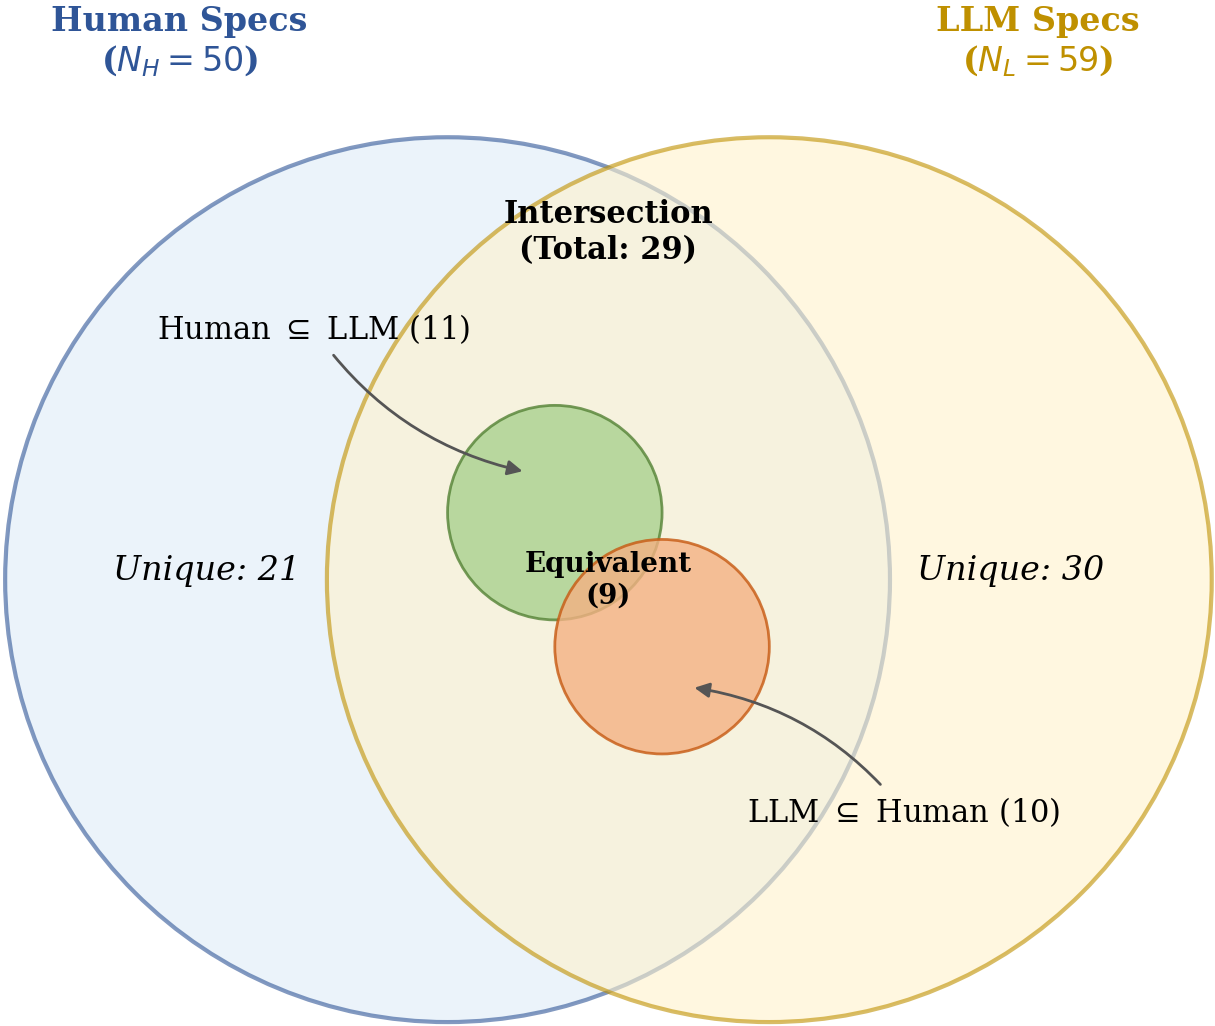
\includegraphics[width=0.55\linewidth]{images/equivalence.png}
    \caption{Equivalence analysis between human ($N_H=50$) and LLM ($N_L=59$) specifications. Among 29 overlapping problems, only 9 yield provably equivalent specifications.}
    \label{fig:equivalence_venn}
\end{figure}

% \paragraph{Equivalence Analysis.}
% Figure~\ref{fig:equivalence_venn} shows the relationship between 50 validated human and 59 LLM specifications. Of 80 unique problems covered, only 29 (37.2\%) have valid specifications from both sources. Within this intersection, only 9 (31.0\%) yield provably equivalent specifications. The remaining 20 cases exhibit asymmetric implication relationships. Manual inspection of 3 asymmetric cases found all semantically equivalent, yet Gemini-3-Pro fails to produce complete proofs—consistent with Finding~\ref{trade-off} that equivalence proving is unsuitable as a primary quality metric.

% The limited overlap between human and LLM successes suggests complementary strengths: they succeed on distinct problem subsets rather than merely differing in capability level, indicating LLM-based specification synthesis remains a challenging open problem.

\paragraph{Equivalence Analysis.}


Figure~\ref{fig:equivalence_venn} shows the relationship between 50 validated human and 59 LLM specifications. Of 80 unique problems covered, only 29 (36.25\%) have valid specifications from both sources. Within this intersection, 9 (31.0\%) yield provably equivalent specifications with both implication directions formally verified, 3 cases succeed in only one direction, and the remaining 17 cases fail to prove either direction. We manually inspected all 3 single-direction cases and confirmed that the specifications are indeed semantically equivalent—the missing direction fails due to prover limitations rather than genuine semantic differences. This confirms Finding~\ref{trade-off} that equivalence proving introduces systematic underestimation and is unsuitable as a primary quality metric.

The limited overlap between human and LLM successes suggests complementary strengths: they succeed on distinct problem subsets rather than merely differing in capability level, indicating LLM-based specification synthesis remains a challenging open problem.
